%% LyX 2.3.2 created this file.  For more info, see http://www.lyx.org/.
%% Do not edit unless you really know what you are doing.
\documentclass[english,notitlepage]{revtex4-1}
\usepackage{tgpagella}
\usepackage{beramono}
\usepackage[T1]{fontenc}
\usepackage[latin9]{inputenc}
\setcounter{secnumdepth}{3}
\usepackage{babel}
\usepackage{amsmath}
\usepackage[unicode=true]
 {hyperref}

\makeatletter

%%%%%%%%%%%%%%%%%%%%%%%%%%%%%% LyX specific LaTeX commands.
%% Because html converters don't know tabularnewline
\providecommand{\tabularnewline}{\\}

%%%%%%%%%%%%%%%%%%%%%%%%%%%%%% User specified LaTeX commands.
\usepackage{tikz}

\makeatother

\usepackage{listings}
\renewcommand{\lstlistingname}{Listing}

\begin{document}
\global\long\def\tht{\vartheta}%
\global\long\def\ph{\varphi}%
\global\long\def\balpha{\boldsymbol{\alpha}}%
\global\long\def\btheta{\boldsymbol{\theta}}%
\global\long\def\bJ{\boldsymbol{J}}%
\global\long\def\bGamma{\boldsymbol{\Gamma}}%
\global\long\def\bOmega{\boldsymbol{\Omega}}%
\global\long\def\d{\text{d}}%
\global\long\def\t#1{\text{#1}}%
\global\long\def\m{\text{m}}%
\global\long\def\v#1{\boldsymbol{#1}}%
\global\long\def\u#1{\underline{#1}}%

\global\long\def\t#1{\mathbf{#1}}%
\global\long\def\bA{\boldsymbol{A}}%
\global\long\def\bB{\boldsymbol{B}}%
\global\long\def\c{\mathrm{c}}%
\global\long\def\difp#1#2{\frac{\partial#1}{\partial#2}}%
\global\long\def\xset{{\bf x}}%
\global\long\def\zset{{\bf z}}%
\global\long\def\qset{{\bf q}}%
\global\long\def\pset{{\bf p}}%

\title{Preconditioned iterations via the Arnoldi method aka incomplete GMRES}
\author{Christopher Albert}
\date{\today}
\maketitle

\section{Preconditioned iterative schemes}

See also http://www.math.vt.edu/people/sturler/LectureNotes/IterMethods\_02.pdf
and Albert, JPCS Varenna 2016 ``Kinetic Modeling''

\subsection{Basics}

Consider a linear system
\begin{equation}
\hat{A}\v x=\v b,\label{eq:Axb}
\end{equation}
where $\v x$ and $\v b$ are vectors of length $N$ and $\hat{A}$
is an invertible linear operator, i.e.
\begin{equation}
\hat{A}(\lambda\v x+\mu\v y)=\lambda\hat{A}\v x+\mu\hat{A}\v y.
\end{equation}
We assume that the matrix representation of as an $N\times N$ is
not given (usually due to the construction of the algorithm and/or
memory requirements for large $N$), but for a given vector $\v x$
there should be an explicit way to obtain $\hat{A}\v x$, e.g. by
a function call. We are thus limited to matrix-free iterative methods
to solve Eq.~(\ref{eq:Axb}). Such methods include direct (Richardson)
iterations, possibly with some preconditioner, the conjugate gradient
method, and the GMRES method.

In particular we are going to consider problems of treating problems
with some ``first guess'' $\v x_{0}$ and a correction $\hat{K}\v x$
depending self-consistently on the final solution, so
\begin{equation}
\v x=\v x_{0}+\hat{K}\v x.\label{eq:xit}
\end{equation}
This means our operator $\hat{A}$ is of the form
\begin{equation}
\hat{A}=(\hat{I}-\hat{K}),
\end{equation}
where $\hat{I}$ is the identity operator, and our equation~(\ref{eq:xit})
in the form of (\ref{eq:Axb}) with $\v b=\v x_{0}$ becomes
\begin{equation}
(\hat{I}-\hat{K})\v x=\v x_{0},\label{eq:ImK}
\end{equation}
so the solution is formally
\begin{equation}
\v x=(\hat{I}-\hat{K})^{-1}\v x_{0}.\label{eq:sol}
\end{equation}


\subsection{Exact solution in the eigenbasis\label{subsec:Exact-solution-in}}

Assume we have have solved the eigenvalue problem for a full-rank
operator $\hat{K}$ and can write
\begin{equation}
\hat{K}=\hat{V}\hat{\Lambda}\hat{V}^{-1},
\end{equation}
where
\begin{equation}
\hat{\Lambda}=\left(\begin{array}{cccc}
\lambda_{1}\\
 & \lambda_{2}\\
 &  & \ddots\\
 &  &  & \lambda_{N}
\end{array}\right)=\v{\Lambda}\hat{I}
\end{equation}
is a diagonal matrix containing eigenvalues, 
\begin{equation}
\hat{V}=(\v v_{1},\v v_{2},\dots\v v_{N})
\end{equation}
is a matrix with respective eigenvectors as columns, and $\hat{V}^{-1}$
is its inverse. For\emph{ normal }matrices the eigenvectors form an
orthogonal basis and $\hat{V}^{-1}$ is equal to the transposed complex
conjugate $\hat{V}^{\ast}$ of $\hat{V}$. Multiplying Eq.~(\ref{eq:ImK})
from the left with $\hat{V}^{-1}$ and defining components $\v x^{\prime}$
in the eigenbasis via
\begin{equation}
\v x=\sum_{k}x_{k}^{\prime}\v v_{k}=(\v v_{1},\v v_{2},\dots\v v_{N})\v x^{\prime}=\hat{V}\v x^{\prime},
\end{equation}
yields an equation

\begin{equation}
(\underbrace{\hat{V}^{-1}\hat{I}\hat{V}}_{\hat{I}}-\hat{\Lambda})\v x^{\prime}=\v x_{0}^{\prime},\label{eq:ImK-1}
\end{equation}
where components of $\v x^{\prime}$ and $\v x_{0}^{\prime}$ in the
eigenbasis $(\v v_{1},\v v_{2},\dots\v v_{N})$ are related to $\v x$
and $\v x_{0}$ in the original canonical basis by the inverse basis
transformation
\begin{equation}
\v x^{\prime}=\hat{V}^{-1}\v x.
\end{equation}
For normal matrices with $\hat{V}^{-1}=\hat{V}^{\ast}$ this reduces
to a projection to eigenvectors
\begin{equation}
\v x^{\prime}=\hat{V}^{\ast}\v x\Rightarrow x_{k}^{\prime}=\v v_{k}^{\star}\cdot\v x.
\end{equation}
In any case we can directly write the solution of Eq.~(\ref{eq:ImK-1})
in the eigenbasis,
\begin{equation}
\v x^{\prime}=(\hat{I}-\hat{\Lambda})^{-1}\v x_{0}^{\prime}=\left(\begin{array}{cccc}
\frac{1}{1-\lambda_{1}}\\
 & \frac{1}{1-\lambda_{2}}\\
 &  & \ddots\\
 &  &  & \frac{1}{1-\lambda_{N}}
\end{array}\right)\left(\begin{array}{c}
x_{01}^{\prime}\\
x_{02}^{\prime}\\
\dots\\
x_{0N}^{\prime}
\end{array}\right).
\end{equation}
Finally we transform back to 
\begin{equation}
\v x=\hat{V}\v x^{\prime}.
\end{equation}

Performing this procedure in an incomplete iterative way until convergence,
starting at the largest eigenvalue using a Krylov/Arnoldi scheme is
known as the GMRES method. Since in the end our matrices will be noisy
and our problems possibly nonlinear, we cannot apply standard method
up to convergence, let alone find all eigenvalues. Instead we will
work partly in the eigenbasis to precondition the problem and solve
the remaining (hopefully highly convergent) part of the problem by
direct iterations discussed below.

\subsection{Direct iterations}

A simple and robust (but often slow) way to solve Eq.~(\ref{eq:ImK})
iteratively is the following. If we apply the operator $\hat{K}$
to $\v x$ and it doesn't change anymore, this means that we have
found a converged solution. Indeed we can expand Eq.~(\ref{eq:ImK})
to an operator series analogous to the well-known geometric series
\begin{equation}
\frac{1}{1-z}=1+z+z^{2}+\dots\label{eq:series1}
\end{equation}
as a so-called \emph{Neumann} or \emph{operator series}
\begin{equation}
(\hat{I}-\hat{K})^{-1}=\hat{I}+\hat{K}+\hat{K}^{2}+\dots,
\end{equation}
where $\hat{K}^{n}\equiv\hat{K}\hat{K}\dots$ means applying the operator
$n$ times. The solution~(\ref{eq:sol}) to Eq.~(\ref{eq:ImK})
is thus given as an infinite series
\begin{equation}
\v x=(\hat{I}-\hat{K})^{-1}=\v x_{0}+\hat{K}\v x_{0}+\hat{K}^{2}\v x_{0}+\dots\label{eq:series2}
\end{equation}
Of course we can do this kind of expansion for any linear system Eq.~(\ref{eq:Axb})
with operator $\hat{A}$ in by defining $\hat{K}\equiv\hat{A}+\hat{I}$,
but in contrast to the natural expansion for problems of the form
(\ref{eq:ImK}), adding and substracting $\hat{I}$ in Eq.~(\ref{eq:Axb})
seems like a rather arbitrary step.

\subsubsection{Convergence and analogy to the complex geometric series}

Now the natural question is, if the series (\ref{eq:series2}) converges,
and if yes, how fast. Let us take again the geometric series~(\ref{eq:series1})
as an example. The function $1/(1-z)$ is the inverse of $1-z$ in
the sense that
\begin{align*}
(1-z)\,\v x & =\v x_{0}\Leftrightarrow\v x=\frac{1}{1-z}\v x_{0}
\end{align*}
and has a well-defined value for any complex number $z\neq1$ (the
corresponding operator would be $\hat{K}=z\hat{I}$). We can easily
check convergence of the series by taking the formula for finite polynomials
\begin{equation}
1+z+z^{2}+\dots+z^{n}=\frac{1-z^{n+1}}{1-z}.\label{eq:series1-2}
\end{equation}
Taking a limit $n\rightarrow\infty$ shows lets $z^{n}$ vanish if
$|z|<1$. If we put in a number with $|z|>1$ the series diverges
and cannot reproduce the correct result $1/(1-z)$. The series representation~(\ref{eq:series1})
is thus said to have a convergence radius $r=1$. In the limiting
case $|z|=1$ we don't get any useful information, but note the following:
\begin{enumerate}
\item At a real $z=1$ the series diverges, but so does $\frac{1}{1-z}$.
\item At purely imaginary $z=i$ the series oscillates around zero
\begin{equation}
1+i-1-i+\dots\label{eq:series1-1}
\end{equation}
but doesn't converge.
\end{enumerate}
Now we can ask the question how fast the series converges, i.e. how
many terms we need to compute in order to get a reasonable approximation.
Take for example $z=0.2$. Then we have the exact result
\begin{equation}
f(z)=\frac{1}{1-z}=\frac{1}{1-0.2}=\frac{1}{0.8}=1.25\,.
\end{equation}
The first few truncated series terms are
\begin{align}
f_{[0]} & =1,\\
f_{[1]} & =1+0.2=1.2,\\
f_{[2]} & =1+0.2+0.04=1.24,\\
f_{[3]} & =1+0.2+0.04+0.008=1.248,\\
 & \vdots\nonumber 
\end{align}
We observe that we reach a very good approximation of $1.25$ quite
fast. Take on the other hand $z=0.8$ with
\begin{equation}
f(z)=\frac{1}{1-z}=\frac{1}{1-0.8}=\frac{1}{0.2}=5\,.
\end{equation}
Then we have
\begin{align}
f_{[0]} & =1,\label{eq:08}\\
f_{[1]} & =1+0.8=1.8,\\
f_{[2]} & =1+0.8+0.64=2.44,\\
f_{[3]} & =1+0.8+0.64+0.008=2.952,\label{eq:08end}\\
 & \vdots\nonumber 
\end{align}
Here convergence is much worse and we would need a lot more iterations
to reach values close to $5$. The reason is that $z=0.8$ is much
closer to $1$ than $z=0.2$, and thus produces a large value when
taking $1/(1-z)$. Our available series terms are always $<1$ and
must shrink even further to converge. The exact value of $1/(1-z)$
can become arbitrarily large for $z\rightarrow1$ and arbitrarily
close to $1$ for $z\rightarrow0$. In fact in the former case we
have infinitely slow convergence due to the mentioned reason, whereas
in the latter case we have the exact solution already in the $0$th
iteration.

\subsection{Enforcing convergence of a series by a transformation}

Now the question is how we can extend our radius of convergence beyond
$1$ and at the same time accelerate convergence for $z<1$ close
to $1$. Let's see what happens if we rescale
\begin{equation}
z\equiv aw,
\end{equation}
with a fixed $a$. Then we have partial sums
\begin{equation}
1+aw+a^{2}w^{2}+\dots+a^{n}w^{n}=\frac{1-a^{n+1}w^{n+1}}{1-aw}.
\end{equation}
Unfortunately this doesn't help us at all, since the convergence radius
of the series in $w$ is now only $1/a$, which gives us the exact
same behavior as of the original series. This will turn out to be
the reason why a relaxation factor for direct iterations doesn't help
us in this class or problems.

What works better for accelerating convergence is replacing 
\begin{equation}
z=aw+d
\end{equation}
 by a linear transformation with generally complex $a$ and $d$,
i.e.
\begin{equation}
\frac{1}{1-z}=\frac{1}{1-aw-d}=\frac{1}{1-d}\frac{1}{1-\frac{aw}{1-d}}=\frac{1}{1-d}\frac{1}{1-\frac{z-d}{1-d}}.
\end{equation}
The inverse transformation is
\begin{equation}
w=\frac{z}{a}-\frac{d}{a}.\label{eq:zw}
\end{equation}
More generally, to accelerate convergence of complex number series
one would use conformal mappings (see e.g. \href{http://www.math.wisc.edu/~waleffe/M321/complex.pdf}{http://www.math.wisc.edu/$\sim$waleffe/M321/complex.pdf}),
but for our purpose of treating operators, we limit ourselves to linear
transformations. In that case we obtain a geometric series representation
in $\frac{aw}{1-d}$ as
\begin{align}
\frac{1}{1-z} & =\frac{1}{1-d}\left(1+\frac{aw}{1-d}+\left(\frac{aw}{1-d}\right)^{2}+\dots\right)\\
 & =\frac{1}{1-d}\left(1+\frac{z-d}{1-d}+\left(\frac{z-d}{1-d}\right)^{2}+\dots\right)
\end{align}
that converges for $\left|\frac{aw}{1-d}\right|<1$, i.e.
\begin{equation}
|z-d|<|1-d|.\label{eq:conve}
\end{equation}
Remember that $d$ is complex, so we can really shift the complex
origin around (try drawing it), rather than just subtracting real
numbers from $z$. Let's take $d=0.6$ and $a=1$. Then for our case
$z=0.8$ we obtain 
\begin{equation}
w=\frac{z-d}{a}=0.2
\end{equation}
 and approximations
\begin{align}
f_{[0]} & =\frac{1}{1-d}=\frac{1}{0.4}=2.5,\\
f_{[1]} & =\frac{1}{0.4}\left(1+\frac{0.8}{0.4}\right)=3.75,\\
f_{[2]} & =\frac{1}{0.4}\left(1+\frac{0.2}{0.4}+\left(\frac{0.2}{0.4}\right)^{2}\right)=4.375,\\
f_{[3]} & =\frac{1}{0.4}\left(1+\frac{0.2}{0.4}+\left(\frac{0.2}{0.4}\right)^{2}+\left(\frac{0.2}{0.4}\right)^{3}\right)=4.6875,\\
 & \vdots\nonumber 
\end{align}
This is not quite as good as the case of $z=0.2$, but already much
better than the direct iterations in~(\ref{eq:08}-\ref{eq:08end}).
Of course if we had taken $d=z$ then $f_{[0]}=f$ would have been
the exact solution with guaranteed convergence everywhere (except
trivial $z=0$) due to $0<|1-z|$ in (\ref{eq:conve}).

\subsection{Extension to operator series}

For the the operator series of $(\hat{I}-\hat{K})^{-1}$ things work
in a similar way as for the scalar case $1/(1-z)\equiv(\hat{I}-z\hat{I})^{-1}$
and can be understood in terms of \emph{eigenvalues}. Say we knew
$\v x_{0}$ in the eigenbasis,
\begin{equation}
\v x_{0}=\sum_{k=1}^{N}x_{0k}^{\prime}\v v_{k}=\hat{V}\v x_{0}^{\prime}.\label{eq:eigdecomp}
\end{equation}
Then
\begin{equation}
\hat{K}\v x_{0}=\hat{V}\hat{\Lambda}\hat{V}^{-1}\v x_{0}=\hat{V}\hat{\Lambda}\v x_{0}^{\prime}=\sum_{k=1}^{N}\lambda_{k}x_{0k}^{\prime}\v v_{k}.
\end{equation}
Applying $\hat{K}$ for $n$ times yields
\begin{equation}
\hat{K}^{n}\v x_{0}=(\hat{V}\hat{\Lambda}\hat{V}^{-1})(\hat{V}\hat{\Lambda}\hat{V}^{-1})\dots(\hat{V}\hat{\Lambda}\hat{V}^{-1})\v x_{0}=\hat{V}\hat{\Lambda}^{n}\v x_{0}^{\prime}=\sum_{k=1}^{N}\lambda_{k}^{\,n}x_{0k}^{\prime}\v v_{k}.
\end{equation}
Thus \emph{all} eigenvalues $\lambda_{k}^{\,n}$ where $x_{0k}^{\prime}\neq0$
i.e. for normal matrices with some components $\v v_{k}^{\star}\cdot\v x_{0}$
of $\v v_{k}$ in the excitation $\v x_{0}$, have to fulfil $\lambda_{k}^{\,n}<1$
for convergence of
\begin{equation}
\hat{I}+\hat{K}+\hat{K}^{2}+\dots
\end{equation}
with direct iterations. We summarize this feature of values for $z$
inside the geometric series for $1/(1-z)$ as well as the spectrum
of eigenvalues $\lambda_{k}$ of $\hat{K}$ for the operator series
in a drawing:
\begin{center}
\scalebox{0.66}{%<TpX v="&#9;" TeXFormat="&#9;&#9;&#9;&#9;" PdfTeXFormat="&#9;&#9;&#9;&#9;" ArrowsSize="&#9;&#9;&#9;" StarsSize="&#9;" DefaultFontHeight="&#9;" DefaultSymbolSize="&#9;&#9;" ApproximationPrecision="&#9;&#9;&#9;&#9;" PicScale="&#9;" Border="&#9;" BitmapRes="&#9;&#9;&#9;&#9;&#9;" HatchingStep="&#9;" DottedSize="&#9;&#9;&#9;" DashSize="&#9;" LineWidth="&#9;&#9;&#9;" TeXFigure="&#9;&#9;&#9;&#9;">
%  <circle x="&#9;&#9;" y="&#9;&#9;" d="&#9;&#9;&#9;&#9;&#9;&#9;&#9;"/>
%  <star x="&#9;&#9;" y="&#9;&#9;" d="&#9;&#9;&#9;"/>
%  <star x="&#9;&#9;" y="&#9;&#9;" d="&#9;&#9;&#9;"/>
%  <star x="&#9;&#9;" y="&#9;&#9;" d="&#9;&#9;&#9;"/>
%  <star x="&#9;&#9;" y="&#9;&#9;" d="&#9;&#9;&#9;"/>
%  <star x="&#9;&#9;" y="&#9;&#9;" d="&#9;&#9;&#9;"/>
%  <text x="&#9;&#9;&#9;&#9;" y="&#9;&#9;&#9;&#9;" t="&#9;&#9;&#9;&#9;&#9;&#9;&#9;&#9;" h="&#9;"/>
%  <text x="&#9;&#9;" y="&#9;&#9;" t="&#9;&#9;&#9;&#9;&#9;&#9;&#9;" h="&#9;"/>
%  <star x="&#9;&#9;" y="&#9;&#9;" d="&#9;&#9;&#9;"/>
%  <star x="&#9;&#9;" y="&#9;&#9;" d="&#9;&#9;&#9;"/>
%  <star x="&#9;&#9;" y="&#9;&#9;" d="&#9;&#9;&#9;"/>
%  <star x="&#9;&#9;" y="&#9;&#9;" d="&#9;&#9;&#9;"/>
%  <star x="&#9;&#9;" y="&#9;&#9;" d="&#9;&#9;&#9;"/>
%  <star x="&#9;&#9;" y="&#9;&#9;" d="&#9;&#9;&#9;"/>
%  <star x="&#9;&#9;" y="&#9;&#9;" d="&#9;&#9;&#9;"/>
%  <text x="&#9;&#9;" y="&#9;&#9;" t="&#9;&#9;&#9;&#9;&#9;&#9;&#9;&#9;" h="&#9;"/>
%  <star x="&#9;&#9;&#9;&#9;" y="&#9;&#9;" d="&#9;&#9;&#9;"/>
%  <star x="&#9;&#9;&#9;&#9;" y="&#9;&#9;" d="&#9;&#9;&#9;"/>
%  <star x="&#9;&#9;&#9;&#9;" y="&#9;&#9;" d="&#9;&#9;&#9;"/>
%  <star x="&#9;&#9;&#9;&#9;" y="&#9;&#9;" d="&#9;&#9;&#9;"/>
%  <star x="&#9;&#9;&#9;&#9;" y="&#9;&#9;" d="&#9;&#9;&#9;"/>
%  <star x="&#9;&#9;&#9;&#9;" y="&#9;&#9;" d="&#9;&#9;&#9;"/>
%  <star x="&#9;&#9;&#9;&#9;&#9;" y="&#9;&#9;" d="&#9;&#9;&#9;"/>
%  <star x="&#9;&#9;&#9;&#9;&#9;" y="&#9;&#9;" d="&#9;&#9;&#9;"/>
%  <star x="&#9;&#9;&#9;&#9;&#9;" y="&#9;&#9;" d="&#9;&#9;&#9;"/>
%  <star x="&#9;&#9;" y="&#9;&#9;" d="&#9;&#9;&#9;"/>
%  <star x="&#9;&#9;&#9;&#9;" y="&#9;&#9;&#9;&#9;" d="&#9;&#9;&#9;"/>
%  <line x1="&#9;&#9;" y1="&#9;&#9;" x2="&#9;&#9;" y2="&#9;&#9;&#9;" arr2="&#9;&#9;&#9;"/>
%  <line x1="&#9;&#9;" y1="&#9;&#9;" x2="&#9;&#9;&#9;" y2="&#9;&#9;" arr2="&#9;&#9;&#9;"/>
%  <text x="&#9;&#9;" y="&#9;&#9;&#9;&#9;&#9;" t="&#9;&#9;" h="&#9;"/>
%  <text x="&#9;&#9;&#9;" y="&#9;&#9;&#9;&#9;" t="&#9;&#9;" h="&#9;"/>
%  <star x="&#9;&#9;&#9;&#9;" y="&#9;&#9;&#9;&#9;" d="&#9;&#9;&#9;"/>
%  <star x="&#9;&#9;&#9;&#9;" y="&#9;&#9;&#9;&#9;" d="&#9;&#9;&#9;"/>
%</TpX>
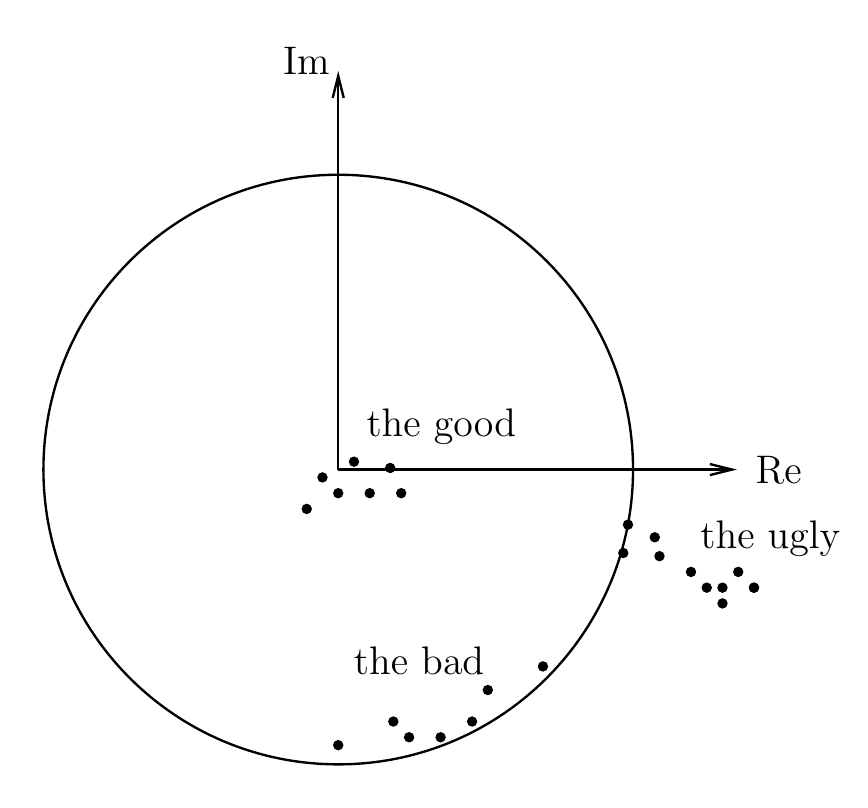
\begin{tikzpicture}[x=1.00mm, y=1.00mm, inner xsep=0pt, inner ysep=0pt, outer xsep=0pt, outer ysep=0pt]
\path[line width=0mm] (10.56,20.56) rectangle +(94.74,95.56);
\definecolor{L}{rgb}{0,0,0}
\path[line width=0.30mm, draw=L] (50.00,60.00) circle (37.44mm);
\definecolor{F}{rgb}{0,0,0}
\path[line width=0.30mm, draw=L, fill=F] (76.00,35.00) circle (0.50mm);
\path[line width=0.30mm, draw=L, fill=F] (50.00,25.00) circle (0.50mm);
\path[line width=0.30mm, draw=L, fill=F] (63.00,26.00) circle (0.50mm);
\path[line width=0.30mm, draw=L, fill=F] (50.00,57.00) circle (0.50mm);
\path[line width=0.30mm, draw=L, fill=F] (52.00,61.00) circle (0.50mm);
\draw(53.60,64.20) node[anchor=base west]{\fontsize{14.23}{17.07}\selectfont the good};
\draw(52.00,34.00) node[anchor=base west]{\fontsize{14.23}{17.07}\selectfont the bad};
\path[line width=0.30mm, draw=L, fill=F] (48.00,59.00) circle (0.50mm);
\path[line width=0.30mm, draw=L, fill=F] (46.00,55.00) circle (0.50mm);
\path[line width=0.30mm, draw=L, fill=F] (54.00,57.00) circle (0.50mm);
\path[line width=0.30mm, draw=L, fill=F] (57.00,28.00) circle (0.50mm);
\path[line width=0.30mm, draw=L, fill=F] (67.00,28.00) circle (0.50mm);
\path[line width=0.30mm, draw=L, fill=F] (69.00,32.00) circle (0.50mm);
\path[line width=0.30mm, draw=L, fill=F] (59.00,26.00) circle (0.50mm);
\draw(96.00,50.00) node[anchor=base west]{\fontsize{14.23}{17.07}\selectfont the ugly};
\path[line width=0.30mm, draw=L, fill=F] (86.80,53.00) circle (0.50mm);
\path[line width=0.30mm, draw=L, fill=F] (94.80,47.00) circle (0.50mm);
\path[line width=0.30mm, draw=L, fill=F] (96.80,45.00) circle (0.50mm);
\path[line width=0.30mm, draw=L, fill=F] (98.80,45.00) circle (0.50mm);
\path[line width=0.30mm, draw=L, fill=F] (90.80,49.00) circle (0.50mm);
\path[line width=0.30mm, draw=L, fill=F] (98.80,43.00) circle (0.50mm);
\path[line width=0.30mm, draw=L, fill=F] (100.80,47.00) circle (0.50mm);
\path[line width=0.30mm, draw=L, fill=F] (102.80,45.00) circle (0.50mm);
\path[line width=0.30mm, draw=L, fill=F] (102.80,45.00) circle (0.50mm);
\path[line width=0.30mm, draw=L, fill=F] (58.00,57.00) circle (0.50mm);
\path[line width=0.30mm, draw=L, fill=F] (56.60,60.20) circle (0.50mm);
\path[line width=0.30mm, draw=L] (50.00,60.00) -- (50.00,110.00);
\path[line width=0.30mm, draw=L, fill=F] (50.00,110.00) -- (49.30,107.20) -- (50.00,110.00) -- (50.70,107.20) -- (50.00,110.00) -- cycle;
\path[line width=0.30mm, draw=L] (50.00,60.00) -- (100.00,60.00);
\path[line width=0.30mm, draw=L, fill=F] (100.00,60.00) -- (97.20,60.70) -- (100.00,60.00) -- (97.20,59.30) -- (100.00,60.00) -- cycle;
\draw(43.00,110.20) node[anchor=base west]{\fontsize{14.23}{17.07}\selectfont Im};
\draw(103.00,58.20) node[anchor=base west]{\fontsize{14.23}{17.07}\selectfont Re};
\path[line width=0.30mm, draw=L, fill=F] (86.20,49.40) circle (0.50mm);
\path[line width=0.30mm, draw=L, fill=F] (90.20,51.40) circle (0.50mm);
\end{tikzpicture}%
}
\par\end{center}

We must get rid of the \emph{ugly} points outside the unit circle
that cause divergence, and would also like to remove \emph{bad} points
close to the inside of the unit circle that cause slow convergence.
With only \emph{good} points left direct iterations will be very fast.

In general we call a method to make an \emph{operator series }converge
by a linear transformation \emph{preconditioned iterations.} More
generally what we have done in the previous section for the seemingly
trivial optimum case $d=z$ is related to the eigenvalues of the operator
where $\hat{K}\v v=\lambda\v v$ for \emph{eigenvectors $\v v$}.
Since for $\hat{K}=z\hat{I}$ all vectors are eigenvectors with $\lambda=z$
the solution becomes trivial in this sense. Now we will extend the
discussed concepts and preconditioning to general linear operators
and their eigenbasis. From section~\ref{subsec:Exact-solution-in}
we already know how to construct an exact solution via the eigenvalue
problem. Now we will only solve a part of the problem in the eigenspace
of the largest eigenvalues for preconditioning. Once we have reached
$\lambda_{k}<1$ (or better $\ll1$) we use direct iterations for
the rest that should rapidly converge if $\lambda_{k}\ll1$. In fact,
for strictly analyzing convergence, one could use the operator norm,
also related to eigenvalues, but here we are satisfied with the more
qualitative explanation and analogy to the complex geometric series.
Krylov/Arnoldi methods are ideally suited for this task, since they
iteratively find the largest eigenvalues (Python and Matlab know this
as ``eigs'' in contrast to the ``eig'' function). In the special
case of Hermitian matrices (they are normal) the Arnoldi method is
known as the Lanczos method.

Let's assume we know the largest $m$ eigenvalues $\lambda_{k}$ of
$\hat{K}$ with eigenvectors $\v v_{k}$, $k=1\dots m$. Then we introduce
the incomplete eigenvector $N\times m$ matrix
\begin{equation}
\hat{V}_{m}=(\v v_{1},\v v_{2},\dots,\v v_{m}).
\end{equation}
Now for a \emph{normal }operator $\hat{K}$ it would be easy to just
project down to the subspace spanned by $\v v_{1\dots m}$ via an
inner product $\v v_{k}^{\star}\cdot\v x$. However, for a general
(not necessarily normal) operator $\hat{K}$ the eigenvectors are
not orthogonal, i.e. $\v v_{i}^{\star}\cdot\v v_{j}\neq|\v v_{j}|^{2}\delta_{ij}$.
This case is similar to the extension of tensor calculus to a general
non-orthogonal basis in co- and contravariant formalism. The case
is handled by the metric tensor components in geometry, that has components
\begin{equation}
g_{ij}=\v e_{i}\cdot\v e_{j}
\end{equation}
and becomes $\delta_{ij}$ in an orthonormal system. We can convert
between co- and contravariant components by $g_{ij}$ and its inverse
matrix $g^{ij}$ for the reciprocal metric. Components of vectors
can be found by projecting to the dual basis, i.e.
\begin{align}
\v a & =\sum_{k}a^{k}e_{k}=\sum_{k}(\v e^{k}\cdot\v a)\v e_{k}\nonumber \\
 & =\sum_{i,k}a_{i}g^{ik}\v e_{k}=\sum_{i,k}(\v e_{i}\cdot\v a)g^{ik}\v e_{k}.
\end{align}
We see that in order to work fully in the usual basis $\v e_{k}$
and avoid the dual basis $\v e^{k}$ we require the reciprocal metric
$g^{ik}$. Also the ``bra-ket'' notation of quantum mechanics works
the same way. Analogously in our complex linear operator space to
be able to project to the partial eigenbasis in $\hat{V}_{m}$ we
define a matrix $\hat{G}_{mm}$ with entries
\begin{equation}
G_{ij}=\v v_{i}^{\star}\cdot\v v_{j}.
\end{equation}
Remember that
\begin{equation}
\v x^{\prime}=\hat{V}^{-1}\v x\label{eq:vinv}
\end{equation}
in a full eigenspace of dimension $N$. Now we cannot get $\hat{V}^{-1}$
of the full eigenspace here but at least project down to the incomplete
eigensubspace spanned by $\hat{V}_{m}$. We split the vector $\v x$
into contributions from the incomplete eigenspace of dimension $m$
and the remaining eigenspace,
\begin{equation}
\v x=\sum_{k=1}^{M}x_{k}^{\prime}\v v_{k}=\sum_{k=1}^{m}x_{k}^{\prime}\v v_{k}+\sum_{k=m+1}^{M}x_{k}^{\prime}\v v_{k}=\hat{V}_{m}\v x_{m}^{\prime}+\hat{V}_{n}\v x_{n}^{\prime}.\label{eq:eigbasis}
\end{equation}

Here we assumed the dimension of the eigenspace to be $N$ and span
the whole space, so the operator $\hat{K}$ must be of full rank.
The eigenvalue equation in full space is 
\begin{equation}
\hat{K}\v v_{k}=\lambda_{k}\v v_{k}
\end{equation}
or
\begin{equation}
\hat{K}\hat{V}=\v{\lambda}\hat{V}=\hat{V}\hat{\Lambda}.
\end{equation}
The reduced eigenvalue equation in $m$ dimensions of the subspace
is
\begin{equation}
\hat{K}\hat{V}_{m}=\v{\lambda}_{m}\hat{V}_{m}=\hat{V}_{m}\hat{\Lambda}_{m}.
\end{equation}
Here the $(m\times m)$ matrix $\hat{\Lambda}_{m}$ must be on the
right-hand side, since $\hat{V}_{m}$ is of size $(N\times m)$.

\begin{table}
\caption{Dimensions of various quantities.}
\begin{tabular}{|c|c|}
\hline 
Quantity & Dimensions\tabularnewline
\hline 
\hline 
$\v x$ & $N\times1$\tabularnewline
\hline 
$\v x_{m}^{\prime}$ & $m\times1$\tabularnewline
\hline 
$\hat{V}_{m}$ & $N\times m$\tabularnewline
\hline 
$\hat{V}_{m}^{\star}$ & $m\times N$\tabularnewline
\hline 
$\hat{G}_{mm}=\hat{V}_{m}^{\star}\hat{V}_{m}$ & $m\times m$\tabularnewline
\hline 
$\v{\lambda}_{m}$ & $1\times m$\tabularnewline
\hline 
$\Lambda_{m}$ & $m\times N$\tabularnewline
\hline 
\end{tabular}
\end{table}

Now let's look at the original equation
\begin{equation}
(\hat{I}-\hat{K})\v x=\v x_{0}.\label{eq:eq}
\end{equation}
We want to find preconditioner of the that should modify (\ref{eq:eq})
to a new equation where the largest $m$ eigenvalues don't contribute
to iterations. Usually this is written by multiplying (\ref{eq:eq})
with the inverse of a full-rank linear operator $\hat{\Pi}^{-1}$
and
\begin{equation}
\hat{\Pi}^{-1}(\hat{I}-\hat{K})\v x=\Pi^{-1}\v x_{0}.\label{eq:precond}
\end{equation}
We choose $\hat{\Pi}^{-1}=\hat{I}-\hat{M}$ with some general $\hat{M}$.
Then Eq.~(\ref{eq:precond}) becomes
\begin{equation}
(\hat{I}-\hat{M}-(\hat{I}-\hat{M})\hat{K})\v x=(\hat{I}-\hat{M})\v x_{0}
\end{equation}
or
\begin{equation}
(\hat{I}+\hat{\bar{K}})\v x=(\hat{I}-\hat{M})\v x_{0}
\end{equation}
with
\begin{align}
\hat{\bar{K}} & =\hat{M}+(\hat{I}-\hat{M})\hat{K}.
\end{align}
Our task to avoid the first $m$ largest eigenvalues of $\hat{K}$
with index $k\leq m$. This means that $\hat{\bar{K}}\v v_{k}\overset{!}{=}0$,
so
\begin{align}
0\overset{!}{=}\hat{\bar{K}}\v v_{k} & =\hat{M}\v v_{k}+(\hat{I}-\hat{M})\lambda_{k}\v v_{k}\nonumber \\
 & =\lambda_{k}\v v_{k}+\hat{M}(1-\lambda_{k})\v v_{k}.
\end{align}
Combining all $\v v_{k}$ inside $\hat{V}_{m}$ equivalently yields
\[
\hat{\bar{K}}\hat{V}_{m}=\hat{V}_{m}\hat{\Lambda}_{m}+\hat{M}\hat{V}_{m}(\hat{I}_{m}-\hat{\Lambda}_{m})\overset{!}{=}0
\]
so
\begin{equation}
\hat{M}\hat{V}_{m}(\hat{\Lambda}_{m}-\hat{I}_{m})\overset{!}{=}\hat{V}_{m}\hat{\Lambda}_{m}.
\end{equation}
Right-multiplying with the inverse of $(\hat{\Lambda}_{m}-\hat{I}_{m})$
yields
\begin{equation}
\hat{M}\hat{V}_{m}\overset{!}{=}\hat{V}_{m}\hat{\Lambda}_{m}(\hat{\Lambda}_{m}-\hat{I}_{m})^{-1}.
\end{equation}
Now we can apply the unity term $(\hat{V}_{m}^{\star}\hat{V}_{m})^{-1}\hat{V}_{m}^{\star}\hat{V}$
to the right-hand side from the right, which gives
\begin{equation}
\hat{M}\hat{V}_{m}\overset{!}{=}\hat{V}_{m}\hat{\Lambda}_{m}(\hat{\Lambda}_{m}-\hat{I}_{m})^{-1}(\hat{V}_{m}^{\star}\hat{V}_{m})^{-1}\hat{V}_{m}^{\star}\hat{V}.
\end{equation}
This trick is similar to expanding the identity operator into bras
and kets in quantum mechanics. Now this equation is for sure solved
by setting
\begin{equation}
\hat{M}\equiv\hat{V}_{m}\hat{\Lambda}_{m}(\hat{\Lambda}_{m}-\hat{I}_{m})^{-1}(\hat{V}_{m}^{\star}\hat{V}_{m})^{-1}\hat{V}_{m}^{\star}.
\end{equation}
The inner part can be grouped to the inverse of an $m$-dimensional
matrix
\begin{equation}
\hat{L}_{mm}\equiv\hat{V}_{m}^{\star}\hat{V}_{m}(\hat{\Lambda}_{m}-\hat{I}_{m})
\end{equation}
that can be used to pre-compute $\hat{L}_{mm}^{-1}$ before iterations
by solving the $m$-dimensional linear system for $m$ right-hand
sides given by the canonical unit vectors $\hat{I}_{m}=(\v e_{1},\v e_{2},\dots\v e_{m})$
in $m$ dimensions,
\begin{equation}
\hat{L}_{mm}\hat{Y}=\hat{I}_{m}.
\end{equation}
and setting $\hat{L}_{mm}^{-1}$ to its solution $\hat{Y}$. Of course
this is only efficient if the number $m$ of large eigenvalues is
much smaller than the total $N$. Finally we write $\hat{M}$ defining
the preconditioner $\hat{\Pi}^{-1}\equiv\hat{I}-\hat{M}$ as
\begin{equation}
\hat{M}\equiv\hat{V}_{m}\hat{\Lambda}_{m}\hat{L}_{mm}^{-1}\hat{V}_{m}^{\star}
\end{equation}
and solve
\[
(\hat{I}-\hat{\bar{K}})\v x=\bar{\v x}_{0}
\]
having the same solution as the original equation, but with stable
and fast iterations in
\begin{equation}
\hat{\bar{K}}=\hat{M}+(\hat{I}-\hat{M})\hat{K}
\end{equation}
with driving term
\begin{equation}
\bar{\v x}_{0}=(\hat{I}-\hat{M})\v x_{0}.
\end{equation}
Note that this is different to the scalar case Eq.~(\ref{eq:zw})
where no concept of eigenvalues exists.

\newpage{}

\begin{lstlisting}[language=Fortran,basicstyle={\ttfamily},showstringspaces=false]
! Arnoldi
print *, "Finding eigenvalues"
ieigen=1
tol = 0.7d0
call arnoldi(nsize, nritz, ritznum, next_iteration)    
do kit = 1, ngrow
   print *, ritznum(kit)
end do

! Here the matrix amat2 = L_mm and a matrix bvec2 = I_mm for 
! multiple right-hand sides when inverting to L_mm is constructed
print *, "Solving subsystem in eigenbasis"
allocate(amat2(ngrow,ngrow),bvec2(ngrow,ngrow),coefren(ngrow))
bvec2=(0.d0,0.d0)
do i=1,ngrow
   bvec2(i,i)=(1.d0,0.d0)
   do j=1,ngrow
      amat2(i,j)=sum(conjg(eigvecs(:,i))*eigvecs(:,j))*(ritznum(j)-(1.d0,0.d0))
   enddo
enddo

! Here amat2*x = bvec is solved, and result x = L_mm^-1 stored in bvec2
call zgesv(ngrow,ngrow,amat2,ngrow,ipiv,bvec2,ngrow,info)

! Preconditioned iterative scheme with Arnoldi
!
! eigvecs(:,1:ngrow) = V_m
! conjg(eigvecs(:,1:ngrow)) = transpose of V_m^\star
! coefren = \Lambda_mm*L_mm^-1*V_m^\star*(Kx - x)
! V_m * coefren = M*(Kx - x) = M*(K - I)*x
!
! Line xnew = xnew - matmul(eigvecs(:,1:ngrow),coefren(1:ngrow)) means
! x_(n+1) = K x_(n) - M*(K - I)*x_(n) = (I - M)*K*x_(n) + M*x_(n) = Kbar*x_(n)
!
xold = (0d0,0d0)
do kit = 1,maxit
   call next_iteration(nsize, xold, xnew)
     
   do j=1,ngrow
      coefren(j)=ritznum(j)*sum(bvec2(j,:)                           &
           *matmul(transpose(conjg(eigvecs(:,1:ngrow))),xnew-xold))
   enddo
   xnew = xnew - matmul(eigvecs(:,1:ngrow),coefren(1:ngrow))
   xold = xnew 
end do
\end{lstlisting}

\newpage{}

\subsection{Application to self-consistent magnetic fields}

Within kinetic or MHD equilibria we compute magnetic response due
to plasma currents,
\begin{equation}
\delta\v B_{p}=\hat{K}(\delta\v B_{p}+\delta\v B_{v}),\label{eq:k}
\end{equation}
where $\hat{K}=\hat{M}\hat{P}$ first computes plasma currents 
\begin{equation}
\v J_{p}=\hat{P}(\delta\v B_{p}+\delta\v B_{v})\label{eq:equi}
\end{equation}
 from the total field and then Maxwell's equations (Ampere's law)
\begin{equation}
\delta\v B_{p}=\hat{M}\delta\v J_{p}\label{eq:ampi}
\end{equation}
only for the plasma currents that change in each iteration, but not
for the coil currents producing $\delta\v B_{v}$ that remain fixed.
The latter have been already processed before via Biot-Savart, yielding
\begin{equation}
\delta\v B_{v}=\hat{M}\delta\v J_{v}\label{eq:ampi2}
\end{equation}
independently. The combined Maxwell's equations 
\begin{equation}
\delta\v B_{p}+\delta\v B_{v}=\hat{M}(\delta\v J_{p}+\delta\v J_{v})
\end{equation}
are thus fulfilled by superposition of (\ref{eq:ampi}) and (\ref{eq:ampi2})

For direct iterations solving Eq.~(\ref{eq:k}) we use the fixed-point
equation
\begin{equation}
\delta\v B_{p}=\hat{K}(\delta\v B_{v}+\delta\v B_{p})=\hat{K}(\delta\v B_{v}+\hat{K}(\delta\v B_{v}+\delta\v B_{p}))=\dots,\label{eq:k-1}
\end{equation}
iterations
\begin{align}
\delta\v B_{p}^{[0]} & =\delta\v B_{v},\\
\delta\v B_{p}^{[1]} & =\hat{K}\delta\v B_{p}^{(0)}=\hat{K}\delta\v B_{v}\\
\delta\v B_{p}^{[n+1]} & =\hat{K}(\delta\v B_{v}+\delta\v B_{p}^{[n]}).
\end{align}
This application of $\hat{K}=\hat{M}\hat{P}$ to the combination of
vacuum field plus previous iteration plus yields \emph{total }results,
where $\delta\v B_{p}^{[n+1]}$ is an already an approximation of
the total $\delta\v B_{p}^{[n+1]}$. This is what the call to \emph{next\_iteration}
in \emph{kin2d.f90 }does with \emph{bnorm\_plas\_prev} = $\delta\v B_{p}^{[n]}$
being computed from plasma currents 
\begin{equation}
\delta\v J_{p}^{[n+1]}=\hat{P}(\delta\v B_{p}^{[n]}+\delta\v B_{v})
\end{equation}
and then fields
\begin{equation}
\delta\v B_{v}^{[n+1]}=\hat{M}\delta\v J_{p}^{[n+1]}.\label{eq:ampi2-1}
\end{equation}
This corresponds to the operator series for $(\hat{I}-\hat{K})$ because
\begin{align}
\delta\v B_{p}^{(n)} & =\hat{K}(\delta\v B_{v}+\delta\v B_{p}^{(n-1)})\nonumber \\
 & =\hat{K}(\delta\v B_{v}+\hat{K}(\delta\v B_{v}+\delta\v B_{p}^{(n-2)}))\nonumber \\
 & =\hat{K}\delta\v B_{v}+\hat{K}^{2}\delta\v B_{v}+\hat{K}^{3}\delta\v B_{v}+\dots+\hat{K}^{n+1}\delta\v B_{v}\nonumber \\
 & =(\hat{I}+\hat{K}+\hat{K}^{2}+\dots+\hat{K}^{n})\hat{K}\delta\v B_{v}.
\end{align}
Here we also call 
\begin{equation}
\v x_{0}=\hat{K}\delta\v B_{v}=\delta\v B_{p}^{[1]}\equiv\delta\v B_{pv}.
\end{equation}
the single-iteration plasma response $\delta\v B_{pv}$ to the vacuum
field $\delta\v B_{v}$. The whole preocedure can also be written
in the \emph{cumulative} way of the operator series described above
by defining differences denoted by parantheses $(n)$ as
\begin{equation}
\delta\v B_{p}^{(n+1)}\equiv\delta\v B_{p}^{[n+1]}-\delta\v B_{p}^{[n]}
\end{equation}
with
\begin{align}
\delta\v B_{p}^{(1)} & =\delta\v B_{p}^{[1]}=\delta\v B_{pv},\\
\delta\v B_{p}^{(n+1)} & =\hat{K}\delta\v B_{p}^{(n)}
\end{align}
and
\begin{equation}
\delta\v B_{p}^{[n]}=\sum_{k=1}^{n}\delta\v B_{p}^{(k)}.
\end{equation}
The correspondence to our operator series in $\hat{K}$ of these quantities
is for
\begin{align}
\v x & \equiv\delta\v B_{p},\\
\v x_{0} & =\delta\v B_{pv}.
\end{align}
where Eq.~(\ref{eq:k}) becomes of the form (\ref{eq:eq}) with
\begin{equation}
(\hat{I}-\hat{K})\delta\v B_{p}=\delta\v B_{pv}.\label{eq:k-2}
\end{equation}
A preconditioned iteration scheme defines an equivalent equation
\begin{equation}
(\hat{I}-\hat{\bar{K}})\delta\v B_{p}=\delta\bar{\v B}_{pv}
\end{equation}
with a new iteration rule
\begin{align}
\delta\v B_{p}^{(1)} & =\delta\bar{\v B}_{pv},\\
\delta\v B_{p}^{(n+1)} & =\hat{\bar{K}}\delta\v B_{p}^{(n)}.
\end{align}
Here we repeat the definition based on the largest $m$ eigenvalues
described in the general section above,
\begin{align}
\delta\bar{\v B}_{pv} & =(\hat{I}-\hat{M})\delta\v B_{pv}\\
\hat{\bar{K}} & =(\hat{M}+(\hat{I}-\hat{M})\hat{K}),\\
\hat{M} & =\hat{V}_{m}\hat{\Lambda}_{m}\hat{L}_{mm}^{-1}\hat{V}_{m}^{\star},\\
\hat{L}_{mm} & =\hat{V}_{m}^{\star}\hat{V}_{m}(\hat{\Lambda}_{m}-\hat{I}_{m}).
\end{align}
Then for preconditioned version of total (summed) field iterations
$[n]$ it follows that
\begin{align}
\delta\v B^{[1]} & =\delta\bar{\v B}_{pv}\nonumber \\
\delta\v B_{p}^{[n+1]} & =\delta\bar{\v B}_{pv}+\hat{\bar{K}}\delta\v B_{p}^{[n]}\nonumber \\
 & =(\hat{I}-\hat{M})\hat{K}\delta\v B_{v}+(\hat{M}+(\hat{I}-\hat{M})\hat{K})\delta\v B_{p}^{[n]}\nonumber \\
 & =\hat{K}(\delta\v B_{v}+\delta\v B_{p}^{[n]})-\hat{M}\hat{K}(\delta\v B_{v}+\delta\v B_{p}^{[n]}).
\end{align}
This is the way the algorithm is currently implemented in \emph{kin2d.f90
}and tested in \emph{test\_arnoldi.f90}.

\section{TODOs for the one who continues kinetic equilibria:}

\subsection{Perturbed problem for noisy matrices}

Check how sensitive the method is to random noise in the operator
$\hat{K}$ and possibly find some general rules of applicability.

\subsection{Underdetermined systems}

Extend the method to singular operators $\hat{K}$ with rank $M<N$.
There the eigendecomposition is replaced by a singular value decomposition
that can also rely on Krylov methods.

\subsection{Extension to nonlinear operators}

Extend the method to nonlinear operators.
\end{document}
